\section{Test Case: Built-in Atmosphere Upwelling}
%=================================================

\subsection{Double precision linux results}
%------------------------------------------
The double precision results for the linux system for the built-in atmosphere test case are shown in figure \ref{fig:run_example_built_in_atm_upwelling-dbl}.

\begin{figure}[htp]
  \centering
  \qquad\sffamily\textbf{Verification Example: Built-in Atmosphere Upwelling}\\
  \qquad\sffamily\textbf{Red Hat linux platform; double precision}\\
  \qquad\textsf{LBLRTM v11.3 brightness temperature difference using a locally generated TAPE3}\\
  \includegraphics[bb=85 403 534 558,clip,scale=1.0]{graphics/run_example_built_in_atm_upwelling/dbl.eps}
  \qquad\textsf{LBLRTM v11.3 brightness temperature difference using AER TAPE3}\\
  \includegraphics[bb=85 226 534 381,clip,scale=1.0]{graphics/run_example_built_in_atm_upwelling/dbl.eps}
  \caption{Built-in Atmosphere Test: Comparison of the AER-supplied \texttt{TAPE27\_ex} output to the locally generated \texttt{TAPE27} output for the \textsl{double precision} version of LBLRTM v11.3 running on a Red Hat linux system. \mbox{\textbf{(a)} Using} a locally generated little-endian \texttt{TAPE3} spectroscopic datafile. \mbox{\textbf{(b)} Using} the AER-supplied little-endian \texttt{TAPE3} spectroscopic datafile.}
  \label{fig:run_example_built_in_atm_upwelling-dbl}
\end{figure}

The most obvious feature in the brightness temperature difference of figure \ref{fig:run_example_built_in_atm_upwelling-dbl} is the ``linear ramp'' from 1000 to approximately 1025\invcm. It is present regardless of which input spectroscopic \texttt{TAPE3} file is used, although for the AER \texttt{TAPE3} the magnitudes are slightly smaller: e.g. at 1000\invcm{} the $\Delta T_B$ for figure \ref{fig:run_example_built_in_atm_upwelling-dbl}(a) is about 25\% larger than that for figure \ref{fig:run_example_built_in_atm_upwelling-dbl}(b). A magnification of this spectral region is shown in figure \ref{fig:run_example_built_in_atm_upwelling-dbl_1000-1025}.

\begin{figure}[htp]
  \centering
  \qquad\sffamily\textbf{Verification Example: Built-in Atmosphere Upwelling}\\
  \qquad\sffamily\textbf{Red Hat linux platform; double precision}\\
  \qquad\textsf{LBLRTM v11.3 brightness temperature difference using a locally generated TAPE3}\\
  \includegraphics[bb=85 403 534 558,clip,scale=1.0]{graphics/run_example_built_in_atm_upwelling/dbl_1000-1025.eps}
  \qquad\textsf{LBLRTM v11.3 brightness temperature difference using AER TAPE3}\\
  \includegraphics[bb=85 226 534 381,clip,scale=1.0]{graphics/run_example_built_in_atm_upwelling/dbl_1000-1025.eps}
  \caption{Built-in Atmosphere Test: A magnification of the 1000-1025\invcm{} spectral region from figure \ref{fig:run_example_built_in_atm_upwelling-dbl}, here using the same y-axis range for both plots. Use of the AER-supplied \texttt{TAPE3} datafile results in smaller residuals. \mbox{\textbf{(a)} Using} a locally generated little-endian \texttt{TAPE3} spectroscopic datafile. \mbox{\textbf{(b)} Using} the AER-supplied little-endian \texttt{TAPE3} spectroscopic datafile.}
  \label{fig:run_example_built_in_atm_upwelling-dbl_1000-1025}
\end{figure}

The other features present in figure \ref{fig:run_example_built_in_atm_upwelling-dbl}, for example the cluster of line residuals around 1040\invcm{}, were thought to be due to differences in how the \texttt{TAPE3} files were generated; such as line strength rejections in the AER-supplied \texttt{TAPE3}. A magnification of these individual lines differences for the locally generated TAPE3 case is shown in figure \ref{fig:run_example_built_in_atm_upwelling-dbl_1035.8-1035.9}. The character of the differences suggest a line width, rather than strength, difference and it is not yet understood how generation of the \texttt{TAPE3} file can influence line width. As no LNFL v2.5 input \texttt{TAPE5} was supplied with the LBLRTM v11.3 distribution, these assumptions need to be confirmed -- or rejected; the different \texttt{TAPE3} file may not be causal.

\begin{figure}[htp]
  \centering
  \qquad\sffamily\textbf{Verification Example: Built-in Atmosphere Upwelling}\\
  \qquad\sffamily\textbf{Red Hat linux platform; double precision}\\
  \qquad\textsf{LBLRTM v11.3 brightness temperature difference using a locally generated TAPE3}\\
  \includegraphics[bb=85 403 534 558,clip,scale=1.0]{graphics/run_example_built_in_atm_upwelling/dbl_1035.8-1035.9.eps}
  \caption{Built-in Atmosphere Test: A magnification of the 1035.8-1035.9\invcm{} spectral region from figure \ref{fig:run_example_built_in_atm_upwelling-dbl}(a) showing the typical residuals seen for the individual ``lines''. The character of the residuals suggests a line width difference.}
  \label{fig:run_example_built_in_atm_upwelling-dbl_1035.8-1035.9}
\end{figure}

An additional feature of figure \ref{fig:run_example_built_in_atm_upwelling-dbl}(b) is barely visible: from 1040 to 1200\invcm{} there appears to be a periodic deviation away from the dashed red zero line. It's difficult to see due to the large y-axis range. A magnification of figure \ref{fig:run_example_built_in_atm_upwelling-dbl}(b) for 1025-1200\invcm{} is shown in figure \ref{fig:run_example_built_in_atm_upwelling-dbl_1025-1200}. The periodicity of the residuals is quite evident -- as is the residual line structure seen superimposed on the periodic differences -- although it must be pointed out that the magnitudes of the residuals are very small.

\begin{figure}[htp]
  \centering
  \qquad\sffamily\textbf{Verification Example: Built-in Atmosphere Upwelling}\\
  \qquad\sffamily\textbf{Red Hat linux platform; double precision}\\
  \qquad\textsf{LBLRTM v11.3 brightness temperature difference using AER TAPE3}
  \includegraphics[bb=80 226 534 381,clip,scale=1.0]{graphics/run_example_built_in_atm_upwelling/dbl_1025-1200.eps}
  \caption{Built-in Atmosphere Test: A magnification of the 1025-1200\invcm{} spectral region from figure \ref{fig:run_example_built_in_atm_upwelling-dbl}(b) showing the periodic residuals.}
  \label{fig:run_example_built_in_atm_upwelling-dbl_1025-1200}
\end{figure}


\subsection{Double precision AIX results}
%----------------------------------------
The double precision results for the AIX system for the built-in atmosphere test case are shown in figure \ref{fig:run_example_built_in_atm_upwelling-dbl_ibm}.

\begin{figure}[htp]
  \centering
  \qquad\sffamily\textbf{Verification Example: Built-in Atmosphere Upwelling}\\
  \qquad\sffamily\textbf{IBM AIX platform; double precision}\\
  \qquad\textsf{LBLRTM v11.3 brightness temperature difference using a locally generated TAPE3}\\
  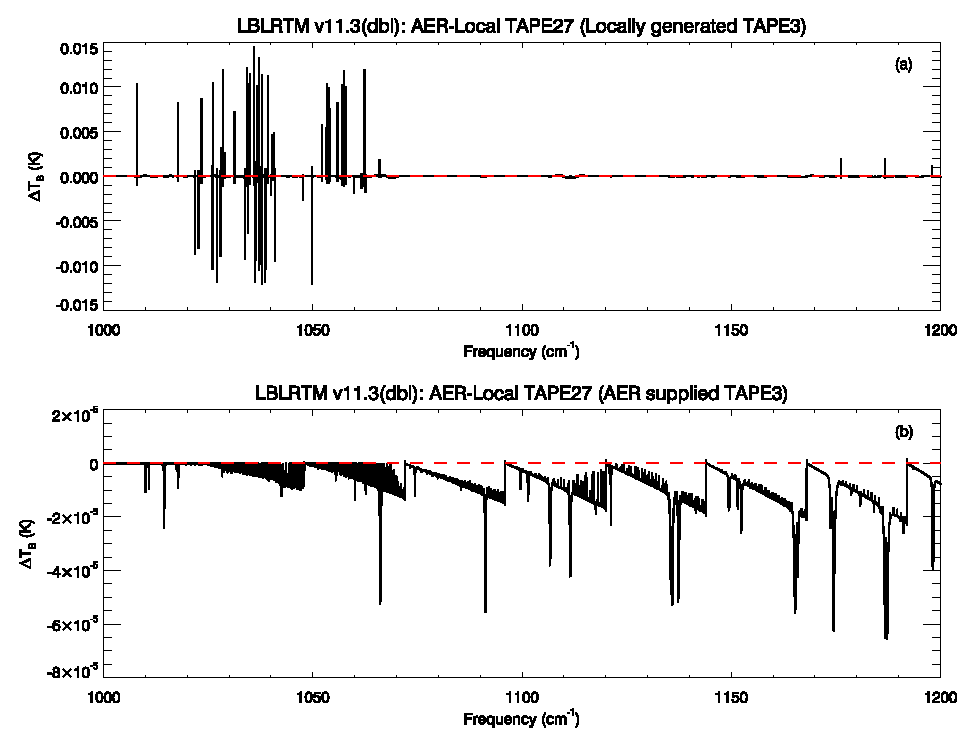
\includegraphics[bb=85 403 534 558,clip,scale=1.0]{graphics/run_example_built_in_atm_upwelling/dbl_ibm.eps}
  \qquad\textsf{LBLRTM v11.3 brightness temperature difference using AER TAPE3}\\
  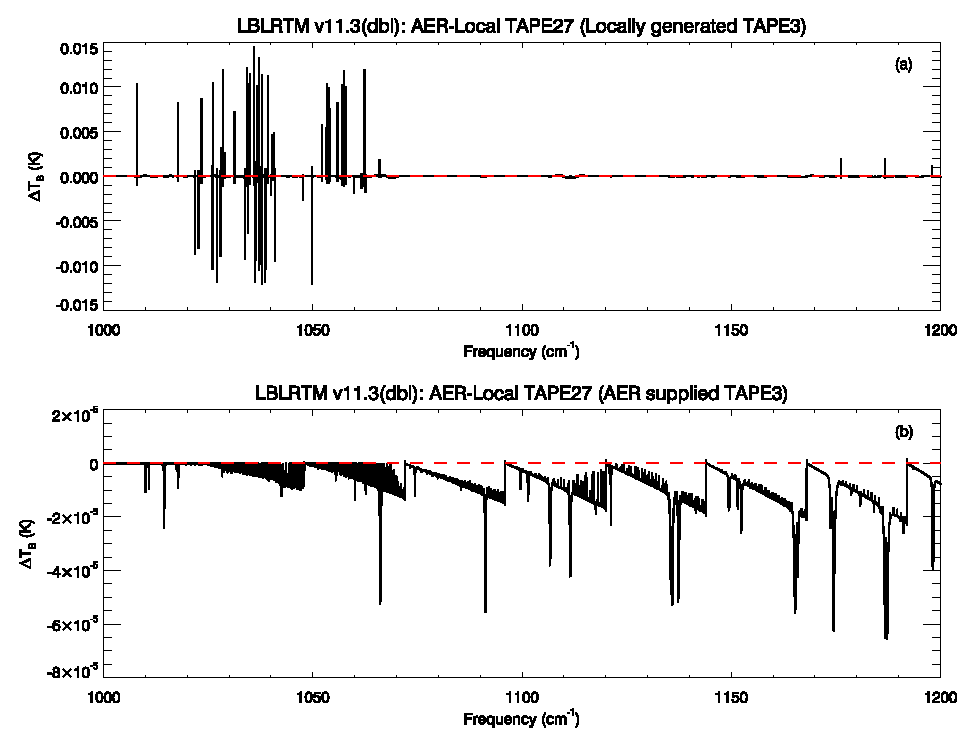
\includegraphics[bb=85 226 534 381,clip,scale=1.0]{graphics/run_example_built_in_atm_upwelling/dbl_ibm.eps}
  \caption{Built-in Atmosphere Test: Comparison of the AER-supplied \texttt{TAPE27\_ex} output to the locally generated \texttt{TAPE27} output for the \textsl{double precision} version of LBLRTM v11.3 running on an IBM AIX system. \mbox{\textbf{(a)} Using} a locally generated big-endian \texttt{TAPE3} spectroscopic datafile. \mbox{\textbf{(b)} Using} the AER-supplied big-endian \texttt{TAPE3} spectroscopic datafile.}
  \label{fig:run_example_built_in_atm_upwelling-dbl_ibm}
\end{figure}

Comparison with the same results for the linux system (figure \ref{fig:run_example_built_in_atm_upwelling-dbl}) shows no ``linear ramp'' residual feature. For the locally generated \texttt{TAPE3} case of figure \ref{fig:run_example_built_in_atm_upwelling-dbl_ibm}(a), the scattered ``line'' differences are almost the same as those seen on in the linux system results of figure \ref{fig:run_example_built_in_atm_upwelling-dbl}(a), and the periodic residuals in \ref{fig:run_example_built_in_atm_upwelling-dbl_ibm}(b) are similar to those highlighted in figure \ref{fig:run_example_built_in_atm_upwelling-dbl_1025-1200} for the linux case.


\subsection{Single precision results}
%------------------------------------
\label{sec:built_in_sgl}
The single precision results for both the linux and AIX systems for the built-in atmosphere test case are shown in figures \ref{fig:run_example_built_in_atm_upwelling-sgl} and \ref{fig:run_example_built_in_atm_upwelling-sgl_ibm} respectively. The two sets of results are effectively identical.

The size of the residuals are, however, slightly disconcerting. These residuals are determined from comparison between the AER-supplied double precision \texttt{TAPE27\_ex} result and the locally generated \texttt{TAPE27} result using a single precision build of LBLRTM v11.3.

\begin{figure}[htp]
  \centering
  \qquad\sffamily\textbf{Verification Example: Built-in Atmosphere Upwelling}\\
  \qquad\sffamily\textbf{Red Hat linux platform; single precision}\\
  \qquad\textsf{LBLRTM v11.3 brightness temperature difference using a locally generated TAPE3}\\
  \includegraphics[bb=85 403 534 558,clip,scale=1.0]{graphics/run_example_built_in_atm_upwelling/sgl.eps}
  \qquad\textsf{LBLRTM v11.3 brightness temperature difference using AER TAPE3}\\
  \includegraphics[bb=85 226 534 381,clip,scale=1.0]{graphics/run_example_built_in_atm_upwelling/sgl.eps}
  \caption{Built-in Atmosphere Test: Comparison of the AER-supplied \texttt{TAPE27\_ex} output to the locally generated \texttt{TAPE27} output for the \textsl{single precision} version of LBLRTM v11.3 running on a Red Hat linux system. \mbox{\textbf{(a)} Using} a locally generated little-endian \texttt{TAPE3} spectroscopic datafile. \mbox{\textbf{(b)} Using} the AER-supplied little-endian \texttt{TAPE3} spectroscopic datafile.}
  \label{fig:run_example_built_in_atm_upwelling-sgl}
\end{figure}

\begin{figure}[htp]
  \centering
  \qquad\sffamily\textbf{Verification Example: Built-in Atmosphere Upwelling}\\
  \qquad\sffamily\textbf{IBM AIX platform; single precision}\\
  \qquad\textsf{LBLRTM v11.3 brightness temperature difference using a locally generated TAPE3}\\
  \includegraphics[bb=85 403 534 558,clip,scale=1.0]{graphics/run_example_built_in_atm_upwelling/sgl_ibm.eps}
  \qquad\textsf{LBLRTM v11.3 brightness temperature difference using AER TAPE3}\\
  \includegraphics[bb=85 226 534 381,clip,scale=1.0]{graphics/run_example_built_in_atm_upwelling/sgl_ibm.eps}
  \caption{Built-in Atmosphere Test: Comparison of the AER-supplied \texttt{TAPE27\_ex} output to the locally generated \texttt{TAPE27} output for the \textsl{single precision} version of LBLRTM v11.3 running on an IBM AIX system. \mbox{\textbf{(a)} Using} a locally generated big-endian \texttt{TAPE3} spectroscopic datafile. \mbox{\textbf{(b)} Using} the AER-supplied big-endian \texttt{TAPE3} spectroscopic datafile.}
  \label{fig:run_example_built_in_atm_upwelling-sgl_ibm}
\end{figure}

So, what is the cause of the relatively large residuals when comparing double and single precision calculations? Magnification of any of the panels of figures \ref{fig:run_example_built_in_atm_upwelling-sgl} or \ref{fig:run_example_built_in_atm_upwelling-sgl_ibm}, as shown in figure \ref{fig:run_example_built_in_atm_upwelling-sgl_1125-1127}, reveals the answer: a frequency shift.

\begin{figure}[htp]
  \centering
  \qquad\sffamily\textbf{Verification Example: Built-in Atmosphere Upwelling}\\
  \qquad\sffamily\textbf{Red Hat linux platform; single precision}\\
  \qquad\textsf{LBLRTM v11.3 brightness temperature difference using AER TAPE3}
  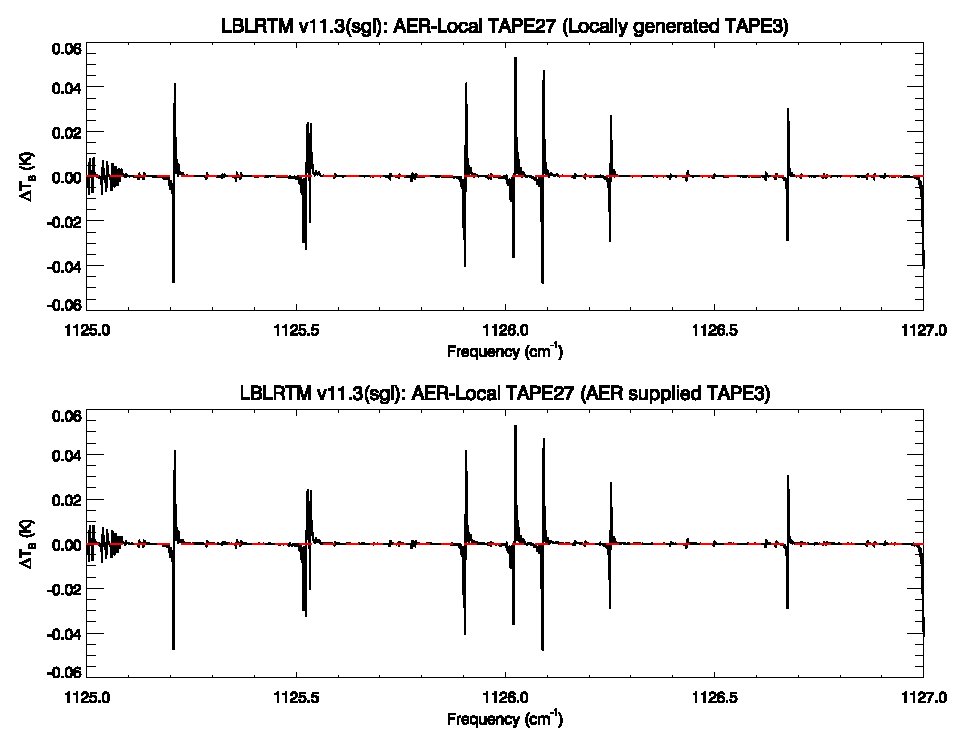
\includegraphics[bb=80 226 534 381,clip,scale=1.0]{graphics/run_example_built_in_atm_upwelling/sgl_1125-1127.eps}
  \caption{Built-in Atmosphere Test: A magnification of the 1125-1127\invcm{} spectral region from figure \ref{fig:run_example_built_in_atm_upwelling-sgl}(b) showing residuals with the characteristic shape due to a frequency shift.}
  \label{fig:run_example_built_in_atm_upwelling-sgl_1125-1127}
\end{figure}

Inspection of the \texttt{TAPE27} (radiance output) and \texttt{TAPE28} (temperature output) datafiles themselves reveals that the frequency shift is in the computed frequencies. Table \ref{tab:tape28_frequency_comparison-sgl} shows sections of computed frequency output from the AER-supplied \texttt{TAPE28\_ex} file and that from the linux system single-precision calculation \texttt{TAPE28} output file. As can be seen, the frequency grids are not the same so differenceing the two values highlights the frequency shift. The magnitude differences seen in the brightness temperatures may be quite reasonable for the frequency shift.

\begin{table}[htp]
  \centering
  \begin{tabular}{r@{.}l r@{.}l c r@{.}l r@{.}l}
    \hline
    \multicolumn{4}{c}{\sffamily\textbf{AER }\texttt{TAPE28\_ex}} & \hspace{1.0cm} & \multicolumn{4}{c}{\sffamily\textbf{Local }\texttt{TAPE28}}\\
    \multicolumn{4}{c}{\sffamily\textbf{(double precision)}} & \hspace{1.0cm} & \multicolumn{4}{c}{\sffamily\textbf{(single precision)}}\\
    \hline
    \multicolumn{2}{c}{\sffamily\textbf{Frequency}} & \multicolumn{2}{c}{\sffamily\textbf{$T_B$}} & \hspace{1.0cm} & \multicolumn{2}{c}{\sffamily\textbf{Frequency}} & \multicolumn{2}{c}{\sffamily\textbf{$T_B$}}\\
    \multicolumn{2}{c}{\sffamily\textbf{(\invcm)}} & \multicolumn{2}{c}{\sffamily\textbf{(K)}} & \hspace{1.0cm} & \multicolumn{2}{c}{\sffamily\textbf{(\invcm)}} & \multicolumn{2}{c}{\sffamily\textbf{(K)}}\\     \hline\hline
     1000&00000000 & 285&17976 & \hspace{1.0cm} & 1000&00000000 & 285&18686 \\
     1000&00024972 & 285&37625 & \hspace{1.0cm} & 1000&00024971 & 285&38333 \\
     1000&00049944 & 285&59329 & \hspace{1.0cm} & 1000&00049942 & 285&60040 \\
     1000&00074915 & 285&78922 & \hspace{1.0cm} & 1000&00074914 & 285&79636 \\
     \multicolumn{4}{c}{\ldots} & & \multicolumn{4}{c}{\ldots}\\
     1099&99958543 & 291&95654 & \hspace{1.0cm} & 1099&99963348 & 291&95667 \\ 
     1099&99983515 & 291&95805 & \hspace{1.0cm} & 1099&99988322 & 291&95816 \\ 
     1100&00008487 & 291&95968 & \hspace{1.0cm} & 1100&00013296 & 291&95975 \\ 
     1100&00033458 & 291&96149 & \hspace{1.0cm} & 1100&00038269 & 291&96158 \\
     \multicolumn{4}{c}{\ldots} & & \multicolumn{4}{c}{\ldots}\\
     1199&99917086 & 292&68271 & \hspace{1.0cm} & 1199&99912876 & 292&68265 \\ 
     1199&99942058 & 292&68505 & \hspace{1.0cm} & 1199&99937849 & 292&68506 \\ 
     1199&99967029 & 292&68725 & \hspace{1.0cm} & 1199&99962822 & 292&68732 \\ 
     1199&99992001 & 292&68910 & \hspace{1.0cm} & 1199&99987795 & 292&68921 \\ 
    \hline
  \end{tabular}
  \caption{Built-in Atmosphere Test: Comparison of tabulated frequencies and brightness temperatures between the AER-supplied \texttt{TAPE28\_ex} output file (calculated in double precision) and the local \texttt{TAPE28} output file (calculated in single precision). The difference in the frequencies, which should always be computed in double precision, is evident.}
  \label{tab:tape28_frequency_comparison-sgl}
\end{table}

This frequency shift was unexpected  since the frequency variables in the LBLRTM source code are always typed as double precision regardless of the compilation switches -- it is conceivable that at some point in the source code, an intermediate frequency calculation involves a default type floating point real variable or literal constant leading to a slight loss in precision for all subsequent calculations. The actual frequency shift spectrum between the double- and single-precision LBLRTM runs is shown in figure \ref{fig:run_example_built_in_atm_upwelling-dbl-sgl_df}.

\begin{figure}[htp]
  \centering
  \qquad\sffamily\textbf{Verification Example: Built-in Atmosphere Upwelling}\\
  \qquad\sffamily\textbf{IBM AIX platform; single precision}\\
  \qquad\textsf{LBLRTM v11.3 double-single precision run frequency difference using AER TAPE3}\\
  \includegraphics[bb=80 403 534 558,clip,scale=1.0]{graphics/run_example_built_in_atm_upwelling/dbl-sgl_df.eps}
  \caption{Built-in Atmosphere Test: The difference in the output \texttt{TAPE27} and \texttt{TAPE28} frequencies between a double- and single-precision LBLRTM v11.3 executable.}
  \label{fig:run_example_built_in_atm_upwelling-dbl-sgl_df}
\end{figure}

